\documentclass[a4paper]{article}
\usepackage{graphicx}
\usepackage[a4paper, margin=2cm]{geometry}
\setlength{\parindent}{0pt}

\title{Lab 4 - Report}
\author{rayane guerou}

\begin{document}

\maketitle


\section{Implementation}
\subsection{Grayscale Image Binarization}
The binarization task was implemented using firstly grayscaling, then we assign white 255 or black 0 pixel depending of the threshold

\begin{figure}[h!]
    \centering
    \includegraphics[scale=0.5]{../src/threshold.png}
    \caption{GPU greyscale 1d}
\end{figure}

\subsection{Brightness Control}
The brightness adjustment was applied by adding a fixed value to each pixel. Values were clipped to the range [0, 255]

\begin{figure}[h!]
    \centering
    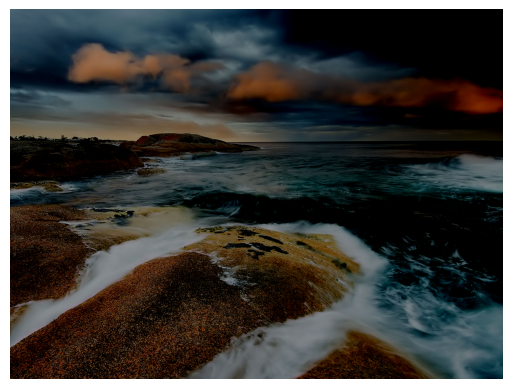
\includegraphics[scale=0.5]{../src/brightness.png}
    \caption{GPU greyscale 1d}
\end{figure}

\subsection{Blending Two Images}
Two images were blended using a weighted sum approach, controlled by an alpha value. The formula used was Q(x, y) = c \times \Phi_1(x, y) + (1 - c) \times \Phi_2(x, y)
With \Phi as the image pixel and c the alpha value

\begin{figure}[h!]
    \centering
    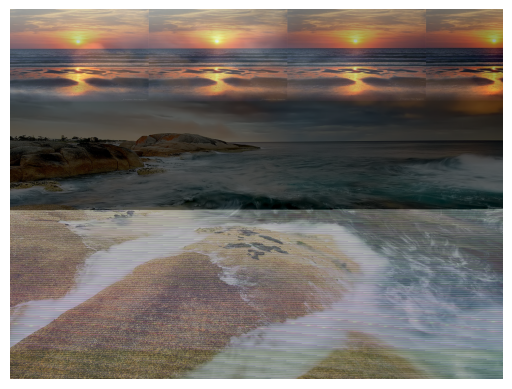
\includegraphics[scale=0.5]{../src/blend.png}
    \caption{GPU greyscale 1d}
\end{figure}

\section{Experiments}
Experiments were conducted with different block sizes (not added for now...)


\end{document}
